\documentclass[12pt]{article}
\usepackage{anyfontsize}
\usepackage[margin = 2cm]{geometry}
\usepackage{polski}
\usepackage[utf8]{inputenc}
\usepackage{tabto}
\usepackage{graphicx}
\usepackage{amsmath}
\usepackage{multicol}
\usepackage{tabularx}
\usepackage{enumitem}
\usepackage{wrapfig}
\usepackage{longtable}
\newcolumntype{L}[1]{>{\raggedright\let\newline\\\arraybackslash\hspace{0pt}}m{#1}}
\newcolumntype{C}[1]{>{\centering\let\newline\\\arraybackslash\hspace{0pt}}m{#1}}



% Dot post number of section
\usepackage{titlesec}
% Underline section, dot post number and span post dot
\titleformat{\section}
    {\Large \bfseries}
    {\thesection.}
    {0.5 cm}
    {}[\titlerule\vspace{0.2cm}]
\titlelabel{\thetitle.\quad}


\usepackage{hyperref}
\hypersetup{
    colorlinks=true,
    linkcolor=black,
    filecolor=magenta,      
    urlcolor=cyan,
    pdfpagemode=FullScreen,
}

\usepackage{listings}
\lstset{
literate=%
    {ą}{{\k{a}}}1
    {Ą}{{\k{A}}}1
    {ć}{{\'c}}1
    {Ć}{{\'{C}}}1
    {ę}{{\k{e}}}1
    {Ę}{{\k{E}}}1
    {ł}{{\l{}}}1
    {Ł}{{\L{}}}1
    {ń}{{\'n}}1
    {Ń}{{\'N}}1
    {ó}{{\'o}}1
    {Ó}{{\'O}}1
    {ś}{{\'s}}1
    {Ś}{{\'S}}1
    {ż}{{\.z}}1
    {Ż}{{\.Z}}1
    {ź}{{\'z}}1
    {Ź}{{\'Z}}1
}


% \usepackage{csvsimple}
% \usepackage{pgfplots}

\usepackage[european, american currents, americanvoltages, RPvoltages, cute inductor]{circuitikz}
\usepackage{tikz}
\usetikzlibrary{shapes.geometric}

\title{\underline{Systemy mikroprocesorowe}\\\textbf{Dokumentacja projektu}\\„Azor” - The czołg}
\author{Łukasz Przystupa,\\ Piotr Kowol}
\date{\today}


\usepackage{titling}
\renewcommand\maketitlehooka{\null\mbox{}\vfill}
\renewcommand\maketitlehookd{\vfill\null}

% \pgfplotsset{compat=1.18}

% \usetikzlibrary{shapes.geometric}


\begin{document}
    \maketitle
    \begin{center}
        Opiekun: Jacek Ostrowski
    \end{center}
    \thispagestyle{empty}
    \newpage


    \section*{Streszczenie}
    \tab Kilka słów podsumowujących pracę. Do napisania na \textbf{koniec}
    \thispagestyle{empty}
    \newpage
    
    \tableofcontents
    \newpage
    \section*{Wstęp}
\phantomsection
\addcontentsline{toc}{section}{\protect\numberline{}Wstęp}
    \tab Też do napisania potem

    \section{Cel i założenia projektowe}
    \tab Powyższy projekt oparty jest o mikrokontroler z rodziny AVR: ATmega8A.
    Komunikując się z odpowiedniki sensorami jest w stanie zlokalizować się w przestrzeni,
    oraz stworzyć prostą mapę pomieszczenia, w którym się znajduje. A następnie swobodnie poruszać się po nim.

    \subsection{Środowisko sprzętowe}
        \tab Jak wyżej wspomniano, sercem projektu jest mikrokontroler ATmega8A, a wspomnianymi modułami są odpowiednio:
        \begin{enumerate}
            \item Ultradźwiękowa czujka odległości -- HC-SR04,
            \item Trój-osiowy akcelerometr -- MMA8451,
            \item Moduł bluetooth -- HC05,
            \item Scalony mostek H -- układ L293D TexasInstruments,
            \item Silniki modelarskie z przekładniami 1:48 o napięciu znamionowym 6V,
            \item Serwo mechanizm -- SG-90,
            \item Trój-osiowy magnetometr QMC5883L.
        \end{enumerate}
% 
        Zasilanie dostarczają dwa wbudowane akumulatory litowo-jonowe 18650 o napięciu znamionowym 3.7V, podniesionym za pomocą przetwornicy STEP UP (CN6009) do około 5V.
        % Zasilanie jest z dwóch akumulatorów litowo-jonowych 18650 o napięciu znamionowym 3.7V, podniesionym za pomocą przetwornicy STEP UP do około 5V.

    \begin{figure}[!ht]
        \centering
        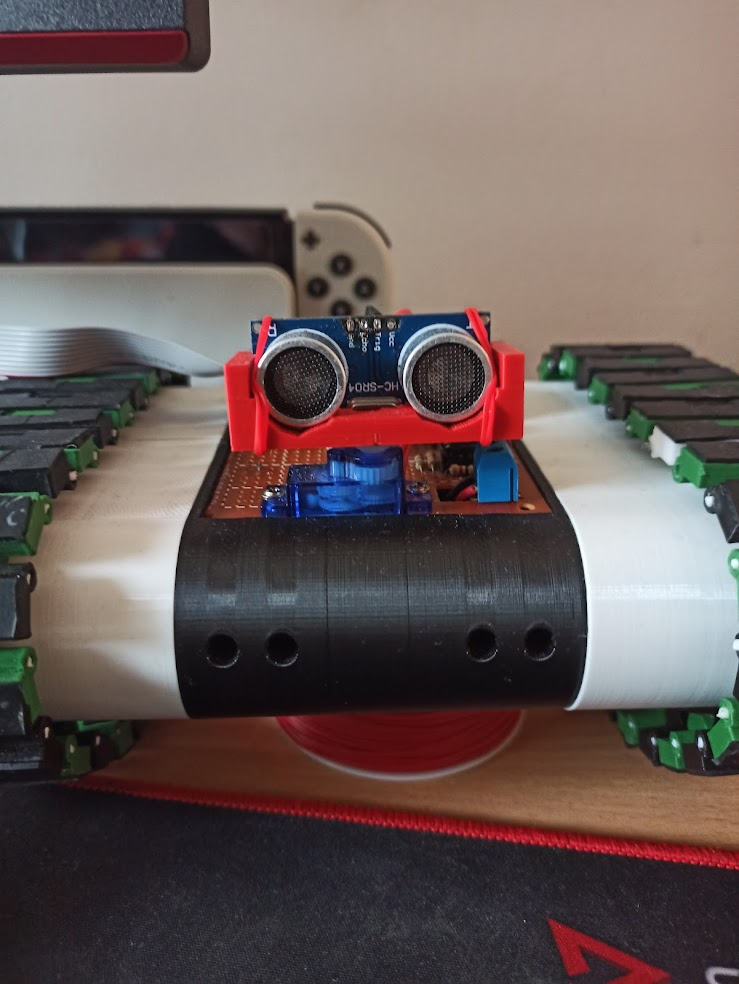
\includegraphics[height = 0.4\textheight]{Img/Azor.jpg}
        \caption{Zdjęcie „Azora”}
    \end{figure}

    \newpage
        \subsubsection{Schemat blokowy}
            \begin{figure}[!h]
    \centering
    \begin{circuitikz}
        \draw
            ( 0,  0) node [draw, rectangle, minimum width = 3cm, minimum height = 8cm](Atmega){ATmega}
            (-5,  1.75) node [draw, rectangle, minimum width = 3cm, minimum height = 2cm](HC_SR04){HC-SR04}
            (-5,  5) node [draw, rectangle, minimum width = 2cm, minimum height = 2cm](bt){HC05}
            ( 7,  1.5) node [draw, rectangle, minimum width = 2cm, minimum height = 2cm](com){QMC5883L}
            ( 7, -1.5) node [draw, rectangle, minimum width = 2cm, minimum height = 2cm](acc){MMA8451}
            ( 5,  4) node [draw, rectangle, minimum width = 2cm, minimum height = 1cm](eeprom){EEPROM}
            ( 5, -4) node [draw, rectangle, minimum width = 2cm, minimum height = 2cm](enkoder){Enkoder}
            
            (-5, -2) node [draw, rectangle, minimum width = 2cm, minimum height = 2cm](H_bridge){H Bridge}
            (-4, -5) node [draw, rectangle, minimum width = 2cm, minimum height = 2cm](servo){SG-90}
            (-7, -1.5) to[L] ++ (0, 1) -- ++ (1, 0) edge[bend left] ++ (0.5, -0.5)
            (-7, -1.5) -- ++ (1, 0)
            (-7, -3.5) to[L] ++ (0, 1) -- ++ (1, 0)
            (-7, -3.5) -- ++ (1, 0) edge[bend right] ++ (0.5, 0.5)

            % (3.25, -7) node [draw, rectangle, minimum width = 4cm, minimum height = 2cm, align=center, text width = 3cm](boostUp){Boost Up CN6009}
            % (-2.5, -7)node [draw, rectangle, minimum width = 2cm, minimum height = 2cm, text width = 2cm, align = center](BMS){Battery controller}
            % (0, -7.5) to[battery, invert] ++ (0, -1) node[ground]{}
            % (0, -7.5) -- ++ (-1.35, 0)
            % (0, -7.5) to[short, *-] ++ (1.3, 0)

            % (BMS) to[short, i=Enable] (boostUp)
            % (boostUp) ++(2, 0) -- ++(0.5, 0) -- ++ (0, 0.5) node[vcc]{$V_{CC}$}

            (eeprom) ++ (-0.5, -0.5) -- ++ (0, -5.5) -- ++ (1.4, 0)
            (eeprom) ++ ( 0,   -0.5) -- ++ (0, -5.0) -- ++ (0.9, 0)

            (com) ++ (-1.15, 0.5) to[short, -*] ++ (-0.85, 0) coordinate(sda)
            (com) ++ (-1.15, 0.0) to[short, -*] ++ (-1.35, 0) coordinate(scl)

            (sda) -- ++ (-1.5, 0) -- ++ (0, 1.5) coordinate(sda)
            (scl) -- ++ (-1.5, 0) -- ++ (0, 1.5) coordinate(scl)
            (sda) to[short] ++ (-2, 0)
            (scl) to[short] ++ (-1.5, 0)
            (sda) ++ (-1.25, 0) node[above]{SDA}
            (scl) ++ (-0.75, 0) node[below]{SCL}

            (sda) to[short, *-] ++ (0, 0.25) to[R] ++ (0, 2) node[vcc]{} ++ (-.25, 0.7) node[left]{$V_{CC}$}
            (scl) to[short, *-] ++ (0, 0.75) to[R] ++ (0, 2) node[vcc]{} ++ (0.25, 0.7) node[right]{$V_{CC}$}

            (bt) ++ (1, 0.25) to[short, i=RxD] ++ (2.00, 0) -- ++ (0, -1.75) -- ++ (0.50, 0)
            (bt) ++ (1,-0.25) to[short, i<_=TxD] ++ (1.75, 0) -- ++ (0, -1.75) -- ++ (0.75, 0)

            (HC_SR04) ++ (1.5, 0.25) to[short, i>=Echo] ++ (2.00, 0)
            (HC_SR04) ++ (1.5,-0.25) to[short, i<_=Trig] ++ (2.00, 0)

            (H_bridge) ++ (1, 0) to[short, i<=$\ $] ++ (1.5, 0) -- ++ (1, 0)

            (H_bridge) ++ (2.25, 0) node[above]{5}
            (H_bridge) ++ (2.25, 0) -- ++ ( 0.1,  0.1)
            (H_bridge) ++ (2.25, 0) -- ++ (-0.1, -0.1)

            (enkoder) ++ (-1, 0) -- ++ (-1, 0) -- ++ (0, 2) to[short, i>=$\ $] ++ (-1.5, 0)
            (servo) ++ (0.5, 1) -- ++ (0, 1) to[short, i<=$\ $] ++ (2, 0)
        ;
    \end{circuitikz}
    \caption{Schemat blokowy}
\end{figure}
    % \newpage
        
    \subsection{Środowisko programowe}
        \tab Program na ATmegę został napisany w języku C/C++, z wykorzystaniem bibliotek udostępnionych przez producenta.
        Do programowania, układu zostało wykorzystane narzędzie \textit{AVRdude} wraz z programatorem \textit{USBasp}.
        Natomiast graficzny interfejs dla komputerów klasy PC, został stworzony w Pythonie, z wykorzystaniem biblioteki ,,Turtle".

    \section{Interfejs komunikacyjny}
    \tab Wiele nowoczesnych urządzeń wykorzystuje rozmaite standardy i interfejsy komunikacyjne do różnych celów.
    Tak samo powyższy projekt wykorzystuje kilka prostych standardów do komunikacji zarówno z użytkownikiem oraz peryferiami.

    \subsection{Standard UART i interfejs bluetooth}
        \tab Podstawowym sposobem komunikacji z użytkownikiem jest protokół UART, wraz z interfejsem Bluetooth.
        Standard komunikacji UART, jest to prosty dwukierunkowy asynchroniczny sposób do przesyłania danych między dwoma urządzeniami.\\
        Opis przykładowej ramki w standardzie UART:
            
        \begin{figure}[!ht]
            \centering
            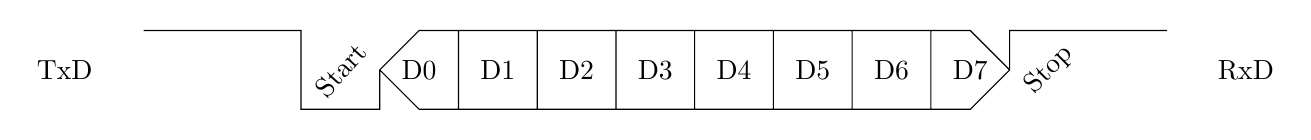
\begin{tikzpicture}
                \draw
                (-1, 0.5) node[]{TxD}
                (0, 1) -- (2, 1)
                    -- (2, 0)
                    -- (3, 0)
                    -- (3, 0.5) coordinate(start) ++(-0.5, 0) node[rotate = 48]{Start}

                (start) --++ (0.5, -0.5) -- ++ (7, 0) --++(0.5, 0.5) coordinate(stop)
                (start) --++ (0.5, 0.5) -- ++ (7, 0) --++(0.5, -0.5)

                (start) ++ (1, 0.5) -- ++ (0, -1) ++ (-0.5, 0.5) node[]{D0}
                (start) ++ (2, 0.5) -- ++ (0, -1) ++ (-0.5, 0.5) node[]{D1}
                (start) ++ (3, 0.5) -- ++ (0, -1) ++ (-0.5, 0.5) node[]{D2}
                (start) ++ (4, 0.5) -- ++ (0, -1) ++ (-0.5, 0.5) node[]{D3}
                (start) ++ (5, 0.5) -- ++ (0, -1) ++ (-0.5, 0.5) node[]{D4}
                (start) ++ (6, 0.5) -- ++ (0, -1) ++ (-0.5, 0.5) node[]{D5}
                (start) ++ (7, 0.5) -- ++ (0, -1) ++ (-0.5, 0.5) node[]{D6}
                (start) ++ (8, 0.5) ++ (0, -1) ++ (-0.5, 0.5) node[]{D7}
                % (start) ++ (8.5, 0) node[]{P}

                (stop) --++(0, 0.5) -- ++(2, 0) coordinate(end)
                (stop) ++ (0.5, 0) node[rotate = 45]{Stop}
                (end) ++ (1, -0.5) node[]{RxD}
                        
                ;
            \end{tikzpicture}
            \caption{Ramka danych w standardzie UART}
        \end{figure}
% 
        \noindent
        W tym projekcie komunikacja odbywa się z szybkością 9600baud'ów (Do zmiany prawie na 100\%).
        Dodatkowo, standard pozwala na przesyłanie dodatkowego bity parzystości ,,doklejanego" do końca wiadomości, jako sposób sprawdzania poprawności wysłanej wiadomości.

        Dalszą częścią kanału transmisyjnego jest przekaźnik bluetooth, który łączy się z komputerem na odpowiednim porcie szeregowym łatwym do oczytania dla programu napisanego na komputerze.
    
    \subsection{Interfejs Two Wire (I²C)}
        \tab Ostatnim interfejsem, wykorzystywanym przez „Azora” jest interfejs I$^2$C -- czyli dwukierunkowa szeregowa magistrala OC z układ Master-Slave.
        Standard ten służy do połączenie urządzeń peryferyjnych z kontrolerem.
        Komunikacja odbywa się w 8bitowych ramkach, z tym że pierwsza ramka zawsze definiuje adres urządzenia docelowego oraz określa kierunek transmisji „do”~lub~„z”~urządzenia.

        \begin{figure}[!ht]
            \centering
            \begin{circuitikz}
                \draw
                    (0, 0) node[draw, rectangle, minimum width = 2cm, minimum height = 2cm](Master){Master}
                    (0, -3.5) node[draw, rectangle, minimum width = 2cm, minimum height = 2cm](Slave1){Slave 1}
                    (2.5, -3.5) node[draw, rectangle, minimum width = 2cm, minimum height = 2cm](Slave2){Slave 2}
                    (5, -3.5) node[draw, rectangle, minimum width = 2cm, minimum height = 2cm](Slave3){Slave 2}

                    (0.25, -1.5) coordinate(clk) -- (5.5, -1.5) ++ (-1, 0) node[above]{$CLK$}
                    (0.25, -1.5) to[short, *-] ++ (0, 0.5) 
                        
                    (-0.25, -2.25) coordinate(sda) -- (5, -2.25) ++ (-1, 0) node[above]{$SDA$}
                    (-0.25, -2.25) to[short, *-] ++ (0, 1.25) 

                    ( 0.25, -1.5) -- ++ (0, -1)
                    (-0.25, -2.25) -- ++ (0, -0.25)
                        
                    (2.75, -1.5) to[short, *-] ++ (0, -1)
                    (2.25, -2.25) to[short, *-] ++ (0, -0.25)

                    (5.5, -1.5) to[short, -] ++ (0, -1)
                    (5.0, -2.25) to[short, -] ++ (0, -0.25)

                    (clk) -- ++ (-2.5, 0) to[R] ++ (0, 2) node[vcc]{+5V}
                    (sda) -- ++ (-3.0, 0) -- ++ (0, 0.75) to[R] ++(0, 2) node[vcc]{+5V}
                ;
            \end{circuitikz}
            \caption{Schemat blokowy magistrali I$^2$C}
        \end{figure}

\newpage
    \subsection{Interfejs SPI}
        % źródło: http://extronic.pl/content/60-kurs-xmega-interfejs-spi
        \tab Procesor bez programu, jest bezużytecznym kawałkiem krzemu dlatego niezwykle istotnym jest zaprogramowanie układu.
        Podstawową metodą programowania układów z rodziny ATmega jest interfejs SPI. 

        \begin{figure}[!ht]
            \centering
            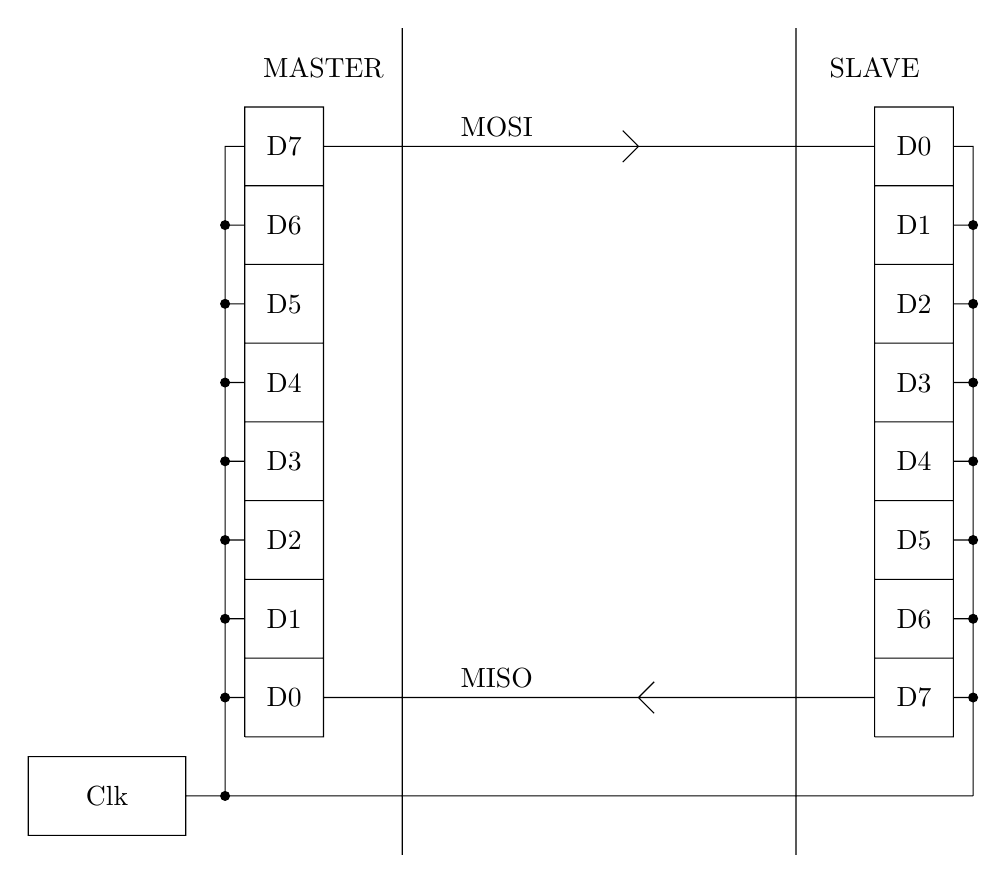
\begin{tikzpicture}
                \draw
                    (0, 0) -- (0, 8) -- (1, 8) -- (1, 0) -- (0, 0)
                    (0, 1) -- (1, 1) ++ (-0.5, -0.5) node[](MD0){D0}
                    (0, 2) -- (1, 2) ++ (-0.5, -0.5) node[]{D1}
                    (0, 3) -- (1, 3) ++ (-0.5, -0.5) node[]{D2}
                    (0, 4) -- (1, 4) ++ (-0.5, -0.5) node[]{D3}
                    (0, 5) -- (1, 5) ++ (-0.5, -0.5) node[]{D4}
                    (0, 6) -- (1, 6) ++ (-0.5, -0.5) node[]{D5}
                    (0, 7) -- (1, 7) ++ (-0.5, -0.5) node[]{D6}
                                        ++       (0, 1) node[](MD7){D7}
                    (2, -1.5) -- (2, 9)

                    (8, 0) -- (8, 8) -- (9, 8) -- (9, 0) -- (8, 0)
                    (8, 1) -- (9, 1) ++ (-0.5, -0.5) node[](SD7){D7}
                    (8, 2) -- (9, 2) ++ (-0.5, -0.5) node[]{D6}
                    (8, 3) -- (9, 3) ++ (-0.5, -0.5) node[]{D5}
                    (8, 4) -- (9, 4) ++ (-0.5, -0.5) node[]{D4}
                    (8, 5) -- (9, 5) ++ (-0.5, -0.5) node[]{D3}
                    (8, 6) -- (9, 6) ++ (-0.5, -0.5) node[]{D2}
                    (8, 7) -- (9, 7) ++ (-0.5, -0.5) node[]{D1}
                                        ++       (0, 1) node[](SD0){D0}
                    (7, -1.5) -- (7, 9)

                        
                    (-2.75, -1.25) rectangle ++ (2, 1)
                    (-1.75, -0.75) node[](clk){Clk} 
                    (clk) ++ (1, 0) coordinate(clk)
                    (clk) -- ++ (0.5, 0)
                        to[short, *-] ++ (0, 1.25) coordinate(MD)
                        to[short, *-] ++ (0.25, 0)
                    (MD) -- ++ (0, 1) coordinate(MD)
                        to[short, *-] ++ (0.25, 0)
                    (MD) -- ++ (0, 1) coordinate(MD)
                        to[short, *-] ++ (0.25, 0)
                    (MD) -- ++ (0, 1) coordinate(MD)
                        to[short, *-] ++ (0.25, 0)
                    (MD) -- ++ (0, 1) coordinate(MD)
                        to[short, *-] ++ (0.25, 0)
                    (MD) -- ++ (0, 1) coordinate(MD)
                        to[short, *-] ++ (0.25, 0)
                    (MD) -- ++ (0, 1) coordinate(MD)
                        to[short, *-] ++ (0.25, 0)
                    (MD) -- ++ (0, 1) coordinate(MD)
                        to[short] ++ (0.25, 0)

                    (clk) -- ++ (10, 0) coordinate(SD)
                    (SD) to[short, -] ++ (0, 1.25) coordinate(SD)
                        -- ++(-0.25, 0)
                    (SD) to[short, *-] ++ (0, 1) coordinate(SD)
                        -- ++(-0.25, 0)
                    (SD) to[short, *-] ++ (0, 1) coordinate(SD)
                        -- ++(-0.25, 0)
                    (SD) to[short, *-] ++ (0, 1) coordinate(SD)
                        -- ++(-0.25, 0)
                    (SD) to[short, *-] ++ (0, 1) coordinate(SD)
                        -- ++(-0.25, 0)
                    (SD) to[short, *-] ++ (0, 1) coordinate(SD)
                        -- ++(-0.25, 0)
                    (SD) to[short, *-] ++ (0, 1) coordinate(SD)
                        -- ++(-0.25, 0)
                    (SD) to[short, *-] ++ (0, 1) coordinate(SD)
                        -- ++(-0.25, 0)

                    (MD7) ++ (0.5, 0) coordinate (MD7)
                    (SD0) ++ (-0.5,0) coordinate (SD0)
                    (MD0) ++ (0.5, 0) coordinate (MD0)
                    (SD7) ++ (-0.5,0) coordinate (SD7)

                    (MD7) -- (SD0)
                    (MD0) -- (SD7)
                        
                    (MD7) ++ (4, 0) -- ++ (-0.2, 0.2)
                    (MD7) ++ (4, 0) -- ++ (-0.2, -0.2)
                    (MD7) ++ (2.2, 0) node[above]{MOSI}
                    % (SD7) ++ (-2.2, 0) node[above]{MISO}

                    (MD0) ++ (4, 0) -- ++ (0.2, 0.2)
                    (MD0) ++ (4, 0) -- ++ (0.2, -0.2)
                    (MD0) ++ (2.2, 0) node[above]{MISO}
                    % (SD0) ++ (-2.2, 0) node[above]{MOSI}

                    (MD7) ++ (0, 1) node[]{MASTER}
                    (SD0) ++ (0, 1) node[]{SLAVE}
                ;

            \end{tikzpicture}
            \caption{Schemat interfejsu SPI}
        \end{figure}
        \noindent
        W przeciwieństwie do poprzednio omawianego interfejsu,
        SPI jest interfejsem typu Master-Slave -- wyróżniamy układ sterujący (Master),
        którego zadaniem jest wyznaczenie taktowania zegara 
        oraz zarządzanie magistralą układami układami podrzędnymi (Slave), poprzez wystawienie stanu aktywnego na pinie \textit{,,CS"}.

        % Dodatkowo, urządzenia slave posiadają specjalne wejście ,,CS", których aktywacja zezwala na komunikację za pomocą protokołu SPI.
        

    \newpage
            

        
            
    \section{Metody pomiarowe}
    \subsection{Odległość -- dalmierz}
        \tab Podstawowym zadaniem „Azora” jest stworzenie mapy tereny.
        Proces ten wykonywany jest za pomocą dalmierza HC-SR04 zamocowane na serwo mechanizmie, dzięki czemu dalmierz może obracać się w osi Z od $0^\circ$ do $180^\circ$.\\
        Schemat połączenia:
        \begin{figure}[!h]
            \centering
            \begin{circuitikz}
                \draw
                    (0, 0) -- (0, -5)
                    (-2, 0) node[]{$\mu P$}

                    (3, -1.75) node[draw, rectangle, minimum width = 2cm, minimum height = 1cm](HC){HC-SR04}
                    (3, -4) node[draw, rectangle, minimum width = 2cm, minimum height = 1cm](SG){SG-90}

                    (0, -1.5) coordinate(ECHO) node[left]{(ECHO) PD4}
                    (0, -2.0) coordinate(TRIG) node[left]{(TRIG) PB6}
                    (0, -4.0) coordinate(PWM)  node[left]{(PWM) PB3}

                    (ECHO) -- ++ (2, 0)
                    (TRIG) -- ++ (2, 0)

                    (PWM) -- ++ (2, 0)

                    (HC) ++ (0, 0.5) node[vcc]{$V_{CC}$}
                    (SG) ++ (0, 0.5) node[vcc]{$V_{CC}$}

                    (HC) ++ (1, 0) node[ground]{}
                ;
            \end{circuitikz}
        \end{figure}

        \subsection{Algorytm działania:}
            \begin{figure}[!h]
                \centering
                \begin{circuitikz}
                    \draw
                        (0, 0) node [draw, circle, minimum width = 2cm, text width = 2cm, align=center]{Wysłanie sygnału TRIG}
                        (0, -4) node[draw, diamond, minimum width= 2cm, text width = 2cm, align=center]{Czy został odebrany sygnał z ECHO}
                    ;
                \end{circuitikz}
            \end{figure}

    \subsection{Prędkość -- enkoder}
    \subsection{Przyspieszenie -- akcelerometr}
    \subsection{Magnetometr -- cyfrowy kompas}
    \section{Interfejs użytkownika}
    \tab Oprogramowanie pozwala na komunikację z „Azorem” oraz reprezentację danych pomiarowych.

    % Po uruchomieniu programu należy z wiersza poleceń wybrać port szeregowy, wykorzystywany do komunikacji przez moduł Bluetooth.
    

    \subsection{Podstawowe sterowanie „Azorem”}
        \tab Podstawowym sposobem sterowania jest interfejs graficzny, który można podzielić na 3 części:

        \subsubsection{Mapa skanowanego obszaru}        
            \tab Największą część okna aplikacji zajmuje mapa skanowanego obszaru, 
            na której czerwonymi liniami zaznaczone są przeszkody a niebieska strzałka reprezentuje „Azora”.

        \subsubsection{Radar}
            \tab Poniżej mapy po lewej stronie znajduje się radar. 
            Którego klikniecie wywołuje funkcję zbierania informacji na temat tego co widzi „Azor” oraz narysowanie ich na mapie. 
            Dodatkowo, na radarze widać aktualną pozycję „głowy Azora”.
        
        \subsubsection{Przyciski sterujące}
            \tab Ostatnią ale nie mniej ważną częścią interfejsu jest 6 strzałek i kulka. 
            Dzięki strzałkom góra/dół można poruszać „Azorem” w przód i w tył.
            Dwie kolejne strzałki w prawo i lewo pozwalają na obrót „Azora” o $90^\circ$.
            Ostatnie dwie strzałeczki odpowiadają za obrót głowy o $15^\circ$, a kuleczka pośrodku odpowiada za wykonanie pojedynczego pomiaru odległości.

    \begin{figure}[!ht]
        \centering
        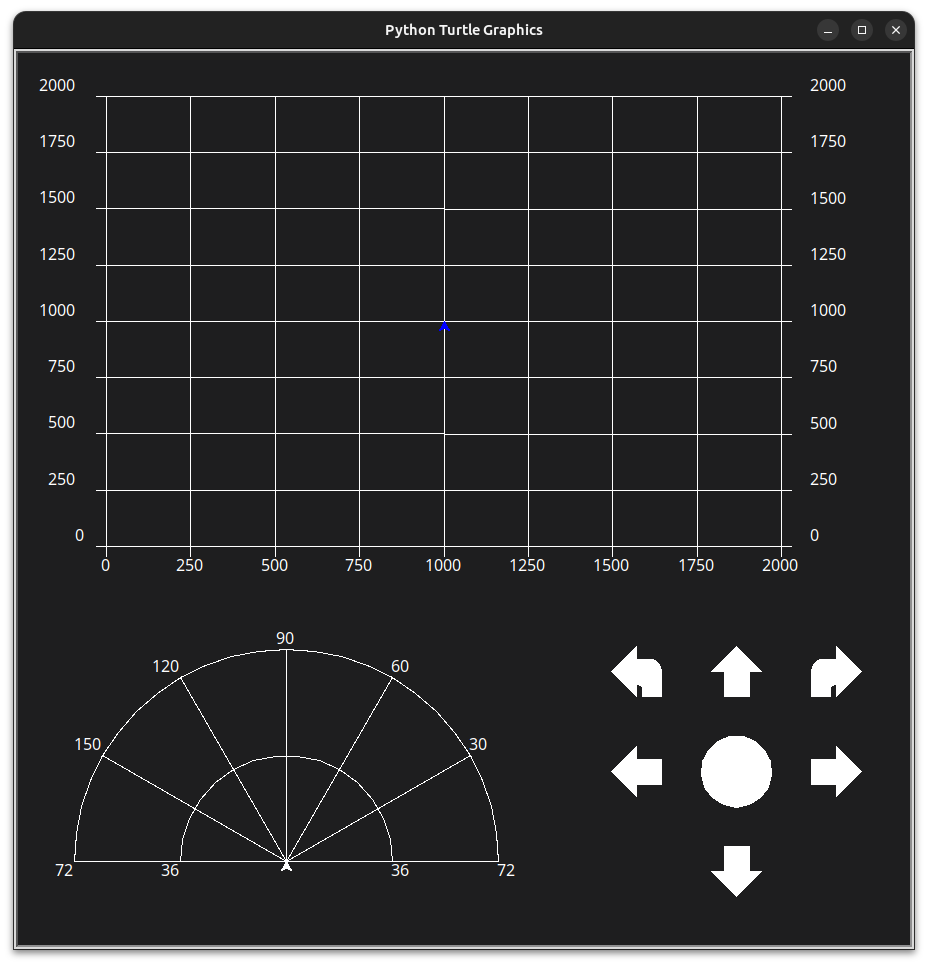
\includegraphics[height = 0.43\textheight]{Img/GUI.png}
        \caption{Interfejs graficzny}
    \end{figure}
        
    
    \newpage
    \subsection{Zaawansowane sterowanie}
        \tab Oprócz sterowania za pomocą przycisków istnieje możliwość wysyłania poleceń do „Azora” za pośrednictwem Command Line'a.
        \begin{figure}[!h]
            \centering
            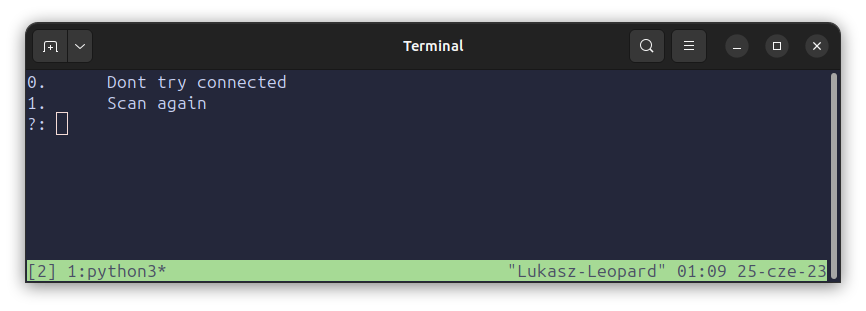
\includegraphics[width = 0.8\textwidth]{Img/CLI.png}
            \caption{Wybór portu do sterowania}
        \end{figure}
        \\Możliwe komendy:
        \begin{itemize}
            \item \textit{forward [wartość]}            - przemieszczenie „Azora” w przód o podaną odległość w mm, domyślna wartość to 100 mm,
            \item \textit{backward [wartość]}           - przemieszczenie „Azora” w tył o podaną odległość w mm, domyślna wartość to 100 mm,
            \item \textit{left [wartość]}               - obrót „Azora” w lewo o podany kąt, wartość domyślna to $90^\circ$,
            \item \textit{right [wartość]}              - obrót „Azora” w prawo o podany kąt, wartość domyślna to $90^\circ$,
            \item \textit{head left/right [wartość]}    - obrót czujnikiem odległości w lewo/prawo o podany kąt,wartość domyślna to $6^\circ$,
            \item \textit{head set [wartość]}           - obrót „głową Azora” do zadanego kąta z zakresu $0^\circ-180^\circ$, domyślnie $90^\circ$, co oznacza „patrzenie” w przód,
            \item \textit{head measure}                 - wykonanie pomiaru odległości dla obecnego ustawienia czujnika odległości,
            \item \textit{acc}                          - zwrócenie aktualnej wartości przyspieszenia na każdej z 3 osi,
            \item \textit{magnet}                       - zwrócenie zmierzonej wartości pola magnetycznego na każdej z 3 osi,
            \item \textit{azimuth}                      - zwrócenie aktualnej wartości azymutu,
            \item \textit{distance}                     - zwrócenie wartości ostatnio pokonanej odległości,
            \item \textit{time}                         - zwrócenie czasu pracy silników,
            \item \textit{velocity}                     - zwrócenie wartości ostatnio zarejestrowanej prędkości,
            \item \textit{radar}                        - wykonanie automatycznego pomiaru odległości w zakresie $0^\circ-180^\circ$ z krokiem $3^\circ$,
            \item \textit{clear}                        - czyszczenie mapy,
            \item \textit{exit}                         - zakończenie działania programu,
        \end{itemize}
    
    \section{Programowanie}
    \tab Do wykorzystania przez użytkownika został oddany jeszcze jeden interfejs kontrolowania „Azora”.
    Jest nim prosty język służy do programowania prostych algorytmów, które Azor ma wykonywać.
    Aby zaprogramować „Azora” należy zamknąć okno interfejsu graficznego oraz zakończyć połączenie z „Azorem”. 
    Następnie należy przejść do folderu „Assembler”, w którym znajdują się dwa skrypty: „compile” oraz „programming”.
    Pierwszy skrypt służy do kompilacji mnemonicznych instrukcji na język wartości zrozumiałe przez interpreter Azora.
    Drugi skrypt wykorzystywany jest do wgrywania programu oraz sprawdzenie czy program wgrał się poprawnie.

    W celu stworzenia własnego programu należy, stworzyć plik tekstowy. Napisać program z pomocą instrukcji zamieszczonych w tabeli poniżej, skompilować go za pomocą komendy:
    \begin{lstlisting}[gobble = 8, frame = L]
        $ python compile.py <nazwa pliku>
    \end{lstlisting}
    oraz wgrać go do Azora za pomocą komendy:
    \begin{lstlisting}[gobble = 8, frame = L]
        $ python programming.py <nazwa pliku>.dec
    \end{lstlisting}


    \subsection{Rejestry}
        \tab Do dowolnego użytku, zostały oddane cztery 16bitowe rejestry: REG0, REG1, REG2, REG3.
        Każdy z podanych rejestrów może zostać w dowolnej instrukcji.
        To znaczy, że każdego rejestru można wykorzystać jako akumulatora, zewnętrznego czy rejestru przesuwnego.
        Znaczną wadą całego układu jest jednak brak możliwości swobodnej migracji danych między rejestrami, autorzy proponują rozwiązanie przedstawione poniżej:
        \begin{lstlisting}[gobble = 8, frame = L, caption={Skopiowanie wartości z Rejestru 0 do Rejestru 1}, captionpos=b]
            PUSH R0 ; zapisanie na stosie wartości z R0
            POP R1  ; Pobranie ze stosu wartości R0 i zapisanie jej w R1
        \end{lstlisting}

    \subsection{Stos}
        \tab Programista, ma możliwość wykorzystania także stosu programowego, o głębokości 16 słów dwu bajtowych.

    \subsection{Pamięć eeprom}
        \tab Ostatnią przestrzenią do magazynowania danych użytkownika jest kość pamięci EEPROM o pojemności 256kB - co odpowiada 128 słowom bitowym.
    
    \newpage
    \begin{table}[!h]
        \centering
        % \vspace{2.5cm}
        \begin{tabularx}{\textwidth}{|c|L{5cm}|>{\centering\arraybackslash}X|>{\centering\arraybackslash}p{1.5cm}|}\hline
            Nr. & Instrukcja & Opis & Bajty\\\hline
             1. & NOP                   & Nic nie rób & 1\\\hline
             2. & END                   & Zakończ wykonywanie programu & 1\\\hline
             3. & SLEEP                 & Usypia procesor i wyłącza wszystkie peryferia* & 1 \\\hline
             4. & ADR\_SET $<reg>$      & Ustaw wskaźnik adresu pamięci & 1 \\\hline
             5. & I2C\_WRITE $<reg>$    & Zapisz do pamięci EEPROM wartość & 1 \\\hline
             6. & I2C\_READ $<reg>$     & Odczyt pamięci EEPROM & 1 \\\hline
             7. & INNER\_READ $<reg>$   & Odczyt pamięci programu & 1 \\\hline
             8. & LDR $<reg>, <val>$    & Zapisz do rejestru wartość & 3 \\\hline
             9. & JUMP\_IF $<reg>,\ <adr>$      & Skocz pod adres jeśli wartość z rejestru $\neq 0$ & 3 \\\hline
            10. & JUMP\_IF\_NOT $<reg>,\ <adr>$ & Skocz pod adres jeśli wartość z rejestru $= 0 $ & 3 \\\hline  
            11. & NOT $<reg>$           & Zaneguj wartość w rejestrze & 1 \\\hline
            12. & ADD $<reg1>,\ <reg2>$ & $reg1 + reg2 = reg1$ & 1 \\\hline
            13. & SUB $<reg1>,\ <reg2>$ & $reg1 - reg2 = reg1$ & 1 \\\hline
            14. & OR  $<reg1>,\ <reg2>$ & $reg1 \wedge  reg2 = reg1$ & 1 \\\hline
            15. & AND $<reg1>,\ <reg2>$ & $reg1 \vee  reg2 = reg1$ & 1 \\\hline
            16. & XOR $<reg1>,\ <reg2>$ & $reg1 \oplus  reg2 = reg1$ & 1 \\\hline
            17. & SHIFT\_LEFT $<reg>$   & Przesuń wartość w rejestrze w lewo o 1 & 1 \\\hline
            18. & SHIFT\_RIGHT $<reg>$  & Przesuń wartość w rejestrze w prawo o 1 & 1\\\hline
            19. & SHIFT\_8\_LEFT $<reg>$ & Przesuń wartość w rejestrze w lewo o 8 & 1 \\\hline
            20. & SHIFT\_8\_RIGHT $<reg>$& Przesuń wartość w rejestrze w prawo o 8 & 1\\\hline
            21. & PUSH $<reg>$          & Wrzuć wartość z rejestru na stos & 1 \\\hline
            22. & POP  $<reg>$          & Zdejmij wartość ze stosu i umieść w rejestrze & 1 \\\hline
            23. & JUMP $<adr>$          & Skod bezwzględnie pod adres & 3 \\\hline
            24. & CALL $<adr>$          & Skocz do funkcji\footnotemark & 3 \\\hline
            25. & RET  $<adr>$          & Wraca z funkcji & 1\\\hline
            26. & INC $<reg>$           & Inkrementuje wartość w rejestrze & 1 \\\hline
            27. & DEC $<reg>$           & Dekementuje wartość w rejestrze & 1 \\\hline
            28. & UART\_READ $<reg>$    & Przeczytaj znak wysłany po serialu & 1 \\\hline
            29. & UART\_SEND $<char>$   & Wyświetl znak z pamięci & 2 \\\hline
            30. & UART\_SEND $<reg>$    & Wyświetl wartość zapisaną w rejestrze & 1 \\\hline
            31. & LED $<reg>$           & Zapal/Zgaś diode & 1 \\\hline
            32. & WAIT $<reg>$          & Poczekaj czas wyrażony w ms & 1 \\\hline
            
            32. & FORWARD               & Uruchom silniki do przodu & 1\\\hline
            33. & BACKWARD              & Uruchom silniki w tył & 1 \\\hline
            34. & TURN $<reg>$        & Obróć pojazd o zadany kąt & 1 \\\hline
            35. & STOP                  & Zatrzymaj silniki & 1 \\\hline

            36. & MEASURE $<reg>$       & Dokonaj pomiaru odległości, wynik zapisz w rejestrze & 1 \\\hline
            37. & ROTATE $<reg>$     & Obróć głową o zadany kąt & 1 \\\hline
            % \multicolumn{4}{|c|}{Instrukcje dla akcelerometru}\\\hline
            % 32. 

        \end{tabularx}
        % \vspace{2.5cm}
        \caption{Tabela instrukcji „Azora”}
    \end{table}
    \footnotetext[1]{Zapisuje na stosie adres powrotu}
    \section{Struktura katalogów i kodu}
    \tab Poniższy rozdział zostanie podzielony na dwie współbieżne sekcje:
    Opis struktury katalogów oraz opis kodu.

    % \subsection{Struktura katalogów}
    \paragraph{Struktura katalogów:\\}
        Projekt ten zawiera się w kilku katalogach, każdy przeznaczony na inną część projektu.
        \begin{itemize}
            \item Assembler,
            \item Docs,
            \item GUI,
            \item Src.
        \end{itemize}

    \subsection{Assembler}
        \tab W powyższym folderze zawarte są pliki do kompilacji programów użytkownika.

        Plik $compile.py$ zawiera skrypt odpowiedzialny za kompilację programu użytkownika.
        Lwią część skryptu zajmuje słownik, z listą instrukcji jako klucze i odpowiadającymi im kodami. 
        Dodatkowo w wartościach słownika przechowywane są informację na temat liczby wykorzystywanych rejestrów oraz ilości dodatkowych bajtów wymaganych przez instrukcję.

        Drugim składnikiem tego katalogu jest skrypt $programming.py$ odpowiedzialny za przeczytanie „skompilowanego” pliku oraz wgranie go do pamięci EEPROM mikrokontrolera.

    \subsection{Docs}
        \tab Drugim w kolejności jest katalog $Docs$, który zawiera kod poniższej dokumentacji.
    
    \subsection{GUI}
        \tab Następnym katalogiem jest folder z graficznym interfejsem użytkownika.
        \begin{itemize}
            \item arrow.py      -- skrypt do rysowania strzałek w GUI,
            \item azor.py       -- skrypt do komunikacji z „Azorem”,
            \item circle.py     -- skrypt do rysowania kulki,
            \item commands.py   -- skrypt do interpretacji komend z CLI,
            \item geometry.py   -- data class z geometrią, poszczególne obiekty korzystają z  tej klasy i w jej obiektach przechowują swoje wymiary i położenie,
            \item GUI.py        -- skrypt zbiorczy do narysowania i rozłożenia obiektów na planszy,
            \item main.py       -- skrypt główny, odpowiedzialny za połączenie CLI i GUI,
            \item map.py        -- skrypt odpowiedzialny za rysowanie mapy terenu,
            \item radar.py      -- skrypt rysowania radaru,
            \item simulation.py -- skrypt zawierający symulację „Azora” w przypadku gdy użytkownik nie ma możliwości połączenia się z oryginałem.
        \end{itemize}
% 
        Dodatkowo w tym katalogu znajduje się jeszcze jeden katalog $Font/$ zawierający czcionkę używaną w GUI.


    \subsection{Src}
        \tab Ostatnim katalogiem jest $Src$, zawierający wszystkie pliki z programem głównym „Azora”. 
        \begin{itemize}
            \item accelerometer*-- obsługa akcelerometru,
            \item coding*       -- switch z programowaniem i wykonywaniem kodu użytkownika,
            \item compass*      -- obsługa kompasu,
            \item eeprom*       -- obsługa pamięci wewnętrznej i zewnętrznej pamięci EEPROM,
            \item engine*       -- obsługa silników,
            \item I2C*          -- biblioteka dodatkowa do I$^2$C,
            \item main          -- główna pętla programu,
            \item PWM*          -- biblioteka pomocnicza do sterowania obrotem „głowy Azora” ,
            \item sonic*        -- obsługa dalmierza - współpracuje z timerem 1,
            \item timer*        -- biblioteka pomocnicza do obsługi timerów i liczników,
            \item uart*         -- biblioteka do komunikacji po USART,
        \end{itemize}
        \vspace{4pt}
        \hrule
        \vspace{16pt}
        \tab * plik podzielony na header $(.hpp)$ i plik źródłowy $(.cpp)$.

    

    % \subsection{Peryferia}
        
    \section{Problemy i rozwiązania}
    \tab Przy tak rozbudowanym projekcie wiele problemów jest nieuniknionych a czas na rozwiązanie, zajmuje ogromne ilości czasu.
    W tym rozdziale zostanie omówione w porządku chronologicznym problemy oraz próby ich rozwiązania lub obejścia.

    \subsection{Zasilanie}
        \tab Pierwszym problemem, na jakie natrafi każdy konstruktor elektroniki przenośnej jest zasilanie własnego urządzenia.
        Nie inaczej było w przypadku „Azora”, pierwszym rozwiązaniem jakie powstało na czas testów była „smycz” od „Azora” do zasilacza laboratoryjnego.
        To rozwiązania jednak szybko okazało sie nieskuteczne -- „Azor był ciągnięty w jedną stronę przez smycz”. 
        Rozwiązaniem więc musiały zostać akumulatory, jednak to niesie za sobą kolejne problemy.

        Pierwszą sprawą do załatwienia jest podniesienie napięcia z $3.7V$ do $5V$. 
        Rozwiązaniem tego problemu jest przetwornica step Up, w projekcie została użyta przetwornica $CN6009$.
        \begin{figure}[!ht]
            \centering
            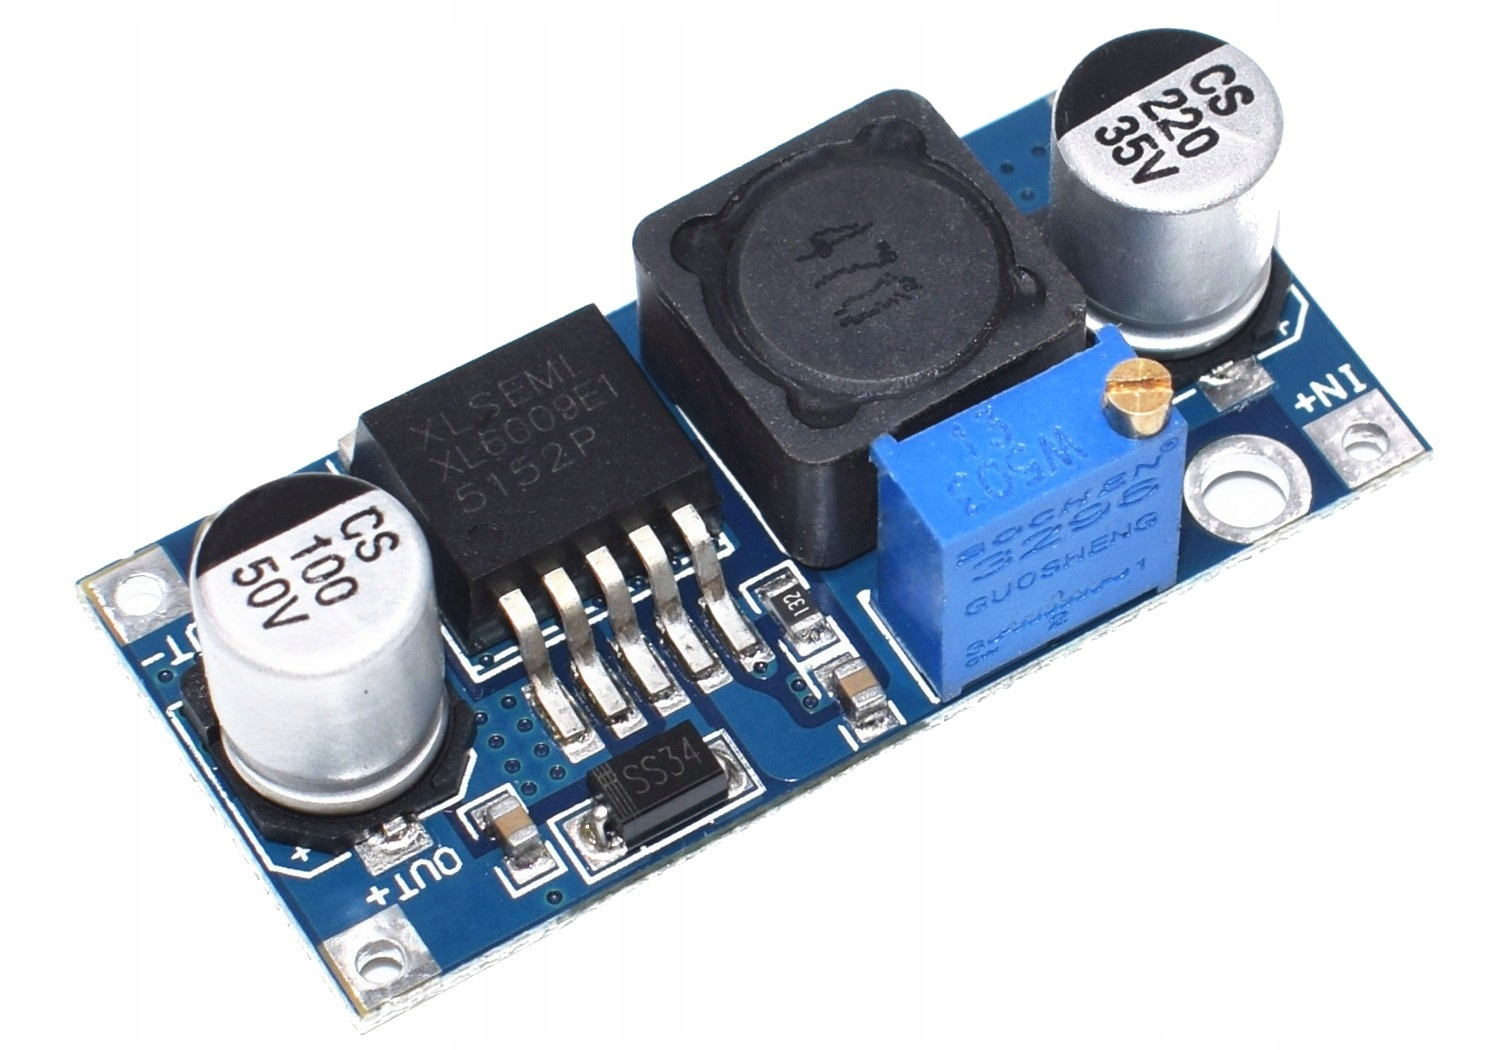
\includegraphics[width = 0.4\textwidth]{Img/przetwornica.jpeg}
            \caption{Zdjęcie modułu z przetwornicą}
        \end{figure}

        \noindent
        Problem wydaje się rozwiązany, napięcie wyjściowe wystarczy ustawić na $5V$ i podłączyć akumulatory.
        Jednak sprawa okazuje się bardziej złożona. 
        Teoretycznie napięcie wejściowe tej przetwornicy dopuszcza minimalną wartość $3V$, jednak producent modułu deklaruje minimalne napięcie pracy o jeden wolt wyższe!
        Kłopotliwa staje sie konstrukcja modułu, w której producent zwarł na stałe napięcie wejściowe i pin Enable przetwornicy, przez co podłączenie napięcia niższego niż $3.5V$ powoduje niestabilną pracę przetwornicy!\\
        Dodatkowo napięcie akumulatorów wcale nie jest napięciem stałym i może zmieniać się od $3.3V - 4.2V$.
        Jednak napięcie $3.3V$ jest minimalnym napięciem pracy! Czyli jest napięciem, którego akumulator \underline{nigdy} nie powinien osiągnąć.

        \newpage
        \textbf{Rozwiązaniem} obu problemów okazuje się prosty obwód detektora progowego na około $3.5V$ przedstawiony na rysunku \ref{schemat:detector}.
        \begin{figure}[!h]
            \centering
            \begin{circuitikz}
                \draw
                    (2, 0) node[op amp, noinv input up, anchor = -](high){lm358}
                    (0, 0) node[op amp, anchor = out, noinv input up](low){lm358}

                    (high.+) to[R, l2_= $R1$ and $11k\Omega$] ++ (0, 2) node[vcc]{Battery}
                    (high.+) to[R, a= $R2$, l= $5k\Omega$, *-] ++ (-2, 0) node[ground]{}

                    (low.out) -- (high.-)
                    (low.-) -- ++(0, -1) coordinate(split) to[R, l=$R3$, a=$10k\Omega$] ++(2.4, 0) to[short, -*] (low.out)
                    (split) to[R, *-, a=$R4$, l=$10k\Omega$] ++ (-2, 0) node[ground]{}

                    (low.+) to[R, l2_=$R5$ and $10k\Omega$] ++ (0, 2) node[vcc]{Battery}
                    (low.+) to[D, *-] ++(-2, 0) node[ground]{}

                    (high.out) to[short, -o] ++(0.5, 0) node[above]{Enable}
                ;
            \end{circuitikz}
            \caption{Schemat detektora}
            \label{schemat:detector}
        \end{figure}

        Istnieje jeszcze jeden problem z tym modułem przetwornicy.
        Gdy spojrzy się na schemat typowego rozwiązania udostępnionego przez producent (rys. \ref{schemat:typ_stepUp}):
        \begin{figure}[!h]
            \centering
            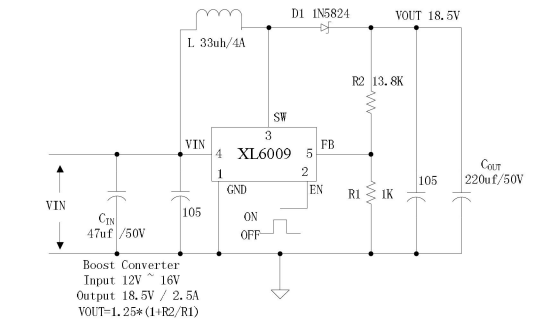
\includegraphics[width = 0.8\textwidth]{Img/prztwornica_schemat.png}
            \caption{Schemat typowej aplikacji przetwornicy}
            \label{schemat:typ_stepUp}
        \end{figure}
        Zauważyć można olbrzymią wadę układu! Diodę \textbf{D1}, która w stanie wyłączenia układu zwiera wejście z wyjściem! 
        Przepuszczając napięcie z akumulatora do układu, pomimo teoretycznie wyłączonego układu!

        \textbf{Rozwiązanie} tego problemu jest MOSFET typu P odcinający zasilanie przetwornicy.
        Jednak ze względu na założenia minimalizacji kosztów, autorzy „wyjęli z szuflady” NMOSa, odcinając za jego pomocą masę układu wykonawczego.


    \subsection{Pomiar prędkości}
        \tab Kolejnym niezwykle trudnym do rozwiązania problemem stał się pomiar prędkości.
        Początkowe założenia, mówiły o pomiarze przyspieszenia i wyliczeniu prędkości (oraz przebytego dystansu) jako całki przyspieszenia w czasie.
        Jednak podczas testów okazało się to praktycznie niewykonalne, o ile czasem udawało się uzyskać sensowne wyniki to w przerażającej większości wyniki były strasznie rozbieżne.
        Przykładowo, podczas ruszania zgodnie z osią $x$ akcelerometru, odczytana wartość przyspieszenia była zgodna co do wartości z teoretyczną wartością jednak jej znak był ujemny!

        \paragraph{Próby rozwiązania\\}
        Autorzy kilkukrotnie rozwiązać ten problem. 
        Jednak żaden ze sposobów nie okazał się dostatecznie dobry.
        Poniżej przedstawiona została lista kilku rozwiązań:
        \begin{enumerate}
            \item Zastosowanie wewnętrznego rejestru FIFO - układ akcelerometru MMA8451Q, posiada do dyspozycji użytkownika wewnętrzny rejestr FIFO pozwalający na zapianie do 32 sampli.
            Jednak włączenie tego rejestru skoków przyspieszenia od wartości dodatnich do wartości ujemnych.
            % 
            \item Debouncing - w nocie katalogowej układu znajduje się możliwość „hardwerowego” debouncingu pomiarów, jednak włączenie tej funkcji w układzie sprawia, że pomiar potrafi nigdy nie dość do skutku przez ciągłe skoki pojazdu na gąsienicach.
            \item Odrzucanie próbek ujemnych - o dziwo, układ akcelerometru bardzo dobrze radzi sobie z określeniem kierunku ruchu! Jednak odrzucenie próbek o przeciwnym znaku niż ten oczekiwany i wyznaczenie z nich średniej wartości prędkości daje w rezultacie totalną bzdurę uparcie zwracając niezerową wartość prędkości pomimo zatrzymania silników!
        \end{enumerate}

        \textbf{Rozwiązaniem} tego problemu w ostateczności zostało pozbycie się akcelerometru.
        W aktualnej wersji projektu, pomiar przemieszczenia odbywa się zgodnie ze sposobem opisanym w sekcji \ref{section:measure:enkoder}.


    \subsection{Obróć się - problematyczny azymut}
        W sekcji \ref{section:measure:azimuth} został opisany sposób pomiary azymutu, na podstawie którego dokonywany jest obrót „Azora” o określony kąt.
        Jednak wartość odchylenia od północy, jaką zwraca uw pomiar, jest wątpliwa.
        Okazuje się, że każdorazowe wyłączenie i włączenie zasilania kompasu, wprowadza nową wartość offsetu w każdej z osi.
        Przez co pomiary konkretnych wartości są niemożliwe do odtworzenia. 

        \paragraph{Rozwiązanie\\}
        Nieskalibrowany moduł zwracał wartości praktycznie losowe, jednak normalizacja wyników, pozwoliła na powtarzalność pomiarów podczas jednego cyklu pracy „Azora”.
        Dodatkową zaletą kalibracji jest możliwość oszacowania różnicy kątów.
        Dzięki tym dwóm zabiegom można obrócić „Azora” o zadany kąt bez przejmowania się dokładnością wyznaczenia północy.
        \begin{align}
            x_{offset} &= \frac{x_{max} + x_{min}}{2}\\
            \overline{\Delta_x} &=  \frac{x_{max} - x_{min}}{2}
        \end{align}
        \begin{align}
            \overline{\Delta} &= \frac{\overline{\Delta_x} + \overline{\Delta_y} + \overline{\Delta_z}}{3}\\
            x_{scale} &= \frac{\overline{\Delta}}{\overline{\Delta_x}}
        \end{align}
        Z pomocą powyższych równań można znormalizować wartości wektorów dla każdej z osi. Ostatnim krokiem w normalizacji jest:
        \begin{equation}
            x = (x_{measure} - x_{offset}) \cdot x_{scale}
        \end{equation}

    \subsection{„Azor poznaje świat” - problem z pomiarem odległości}
        \tab Główną cechą „Azora” jest możliwość  tworzenia mapy terenu na podstawie odległości.
        Jednak co w przypadku gdy pomiar odległości okaże się błędny?
        \begin{figure}[!h]
            \centering
            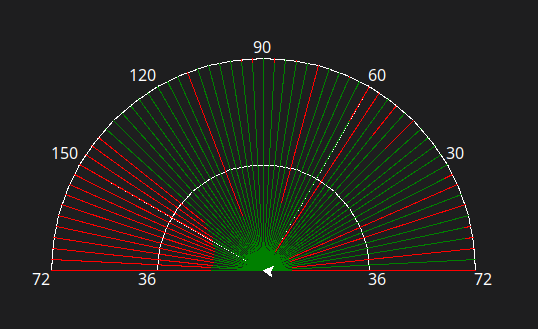
\includegraphics[width = 0.8\textwidth]{Img/radar_error.png}
            \caption{Przykład błędnego odczytu odległości.}
            \label{error:radar_error}
        \end{figure}
        Jak widać na powyższym rysunku \ref{error:radar_error}, kilka pomiarów wychodzi dość dziwnych.
        Na przykład pomiar dla kąta $57^\circ$, znacząco odbiega od pozostałych i tak jest w rzeczywistości jest to zwyczajnie błędny pomiar.

        \paragraph{Rozwiązanie\\}
        Najprostszym sposobem rozwiązania problemu jest wykonanie kilku pomiarów i wyznaczenie średniej.
        Jednak ta metoda nie zawsze się sprawdza.
        Dlatego po wyznaczeniu średniej dla każdego puntu wyznaczana jest wartość pochodnej i jeśli: $r_{i+1} - r_{i-1} = 0$ wtedy wartość $r_i = r_{i-1}$.

\end{document}